\begin{figure}[htbp]
    \centering
    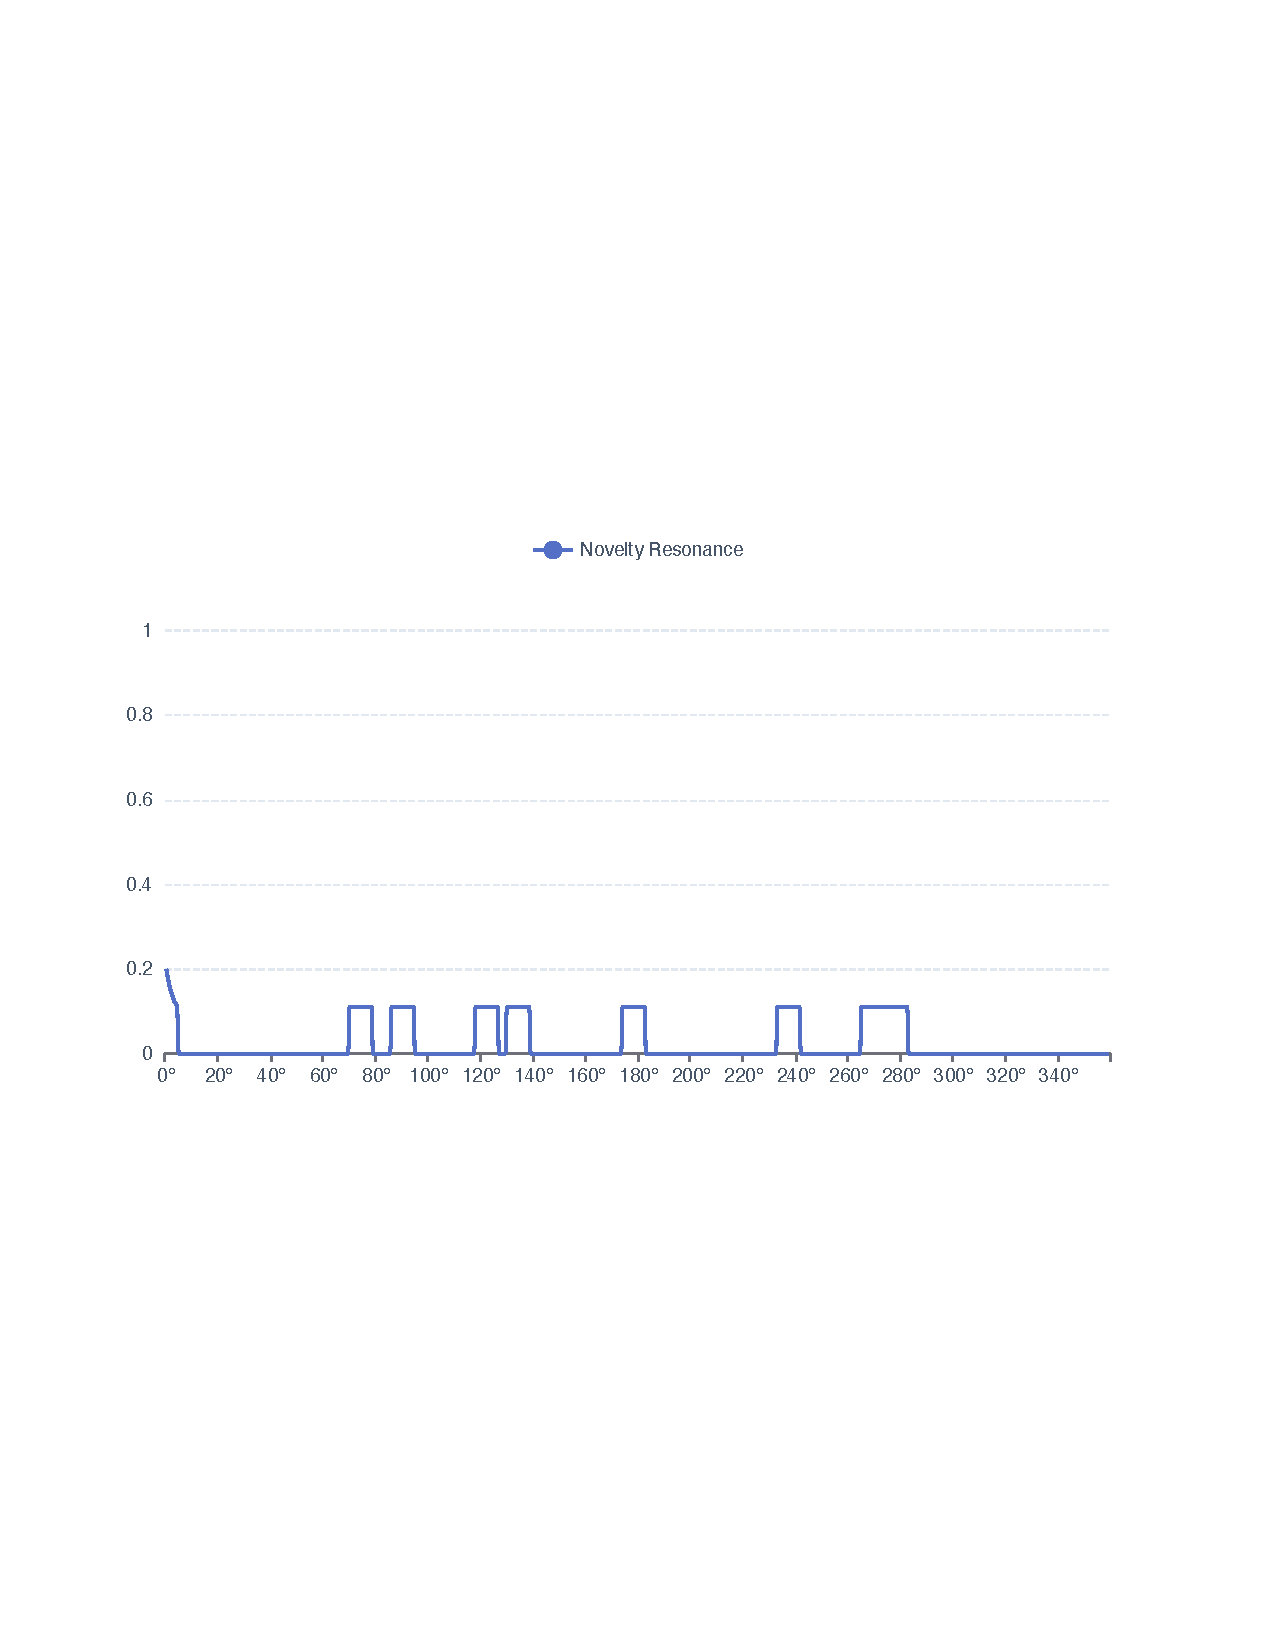
\includegraphics[width=1.0\textwidth]{ permutation_novelty.pdf }
    \caption{ Smoothed rate at which the top-ranked corpus item changes across phase. Two peaks (near 0° and 180°) correspond to the seed and antipodal attractor regions. }
    \label{ fig:permutation_novelty }
\end{figure}
